\documentclass[11pt]{article}
\usepackage[dvipsnames]{xcolor}
\usepackage[T1]{fontenc}
\usepackage{mathtools}
\usepackage[french]{babel}
\usepackage{amsmath,amssymb,amsthm}
\usepackage{framed}
\usepackage{lmodern}
\usepackage{utils}
\usepackage{pdfpages}
\usepackage{irif}


\begin{document}
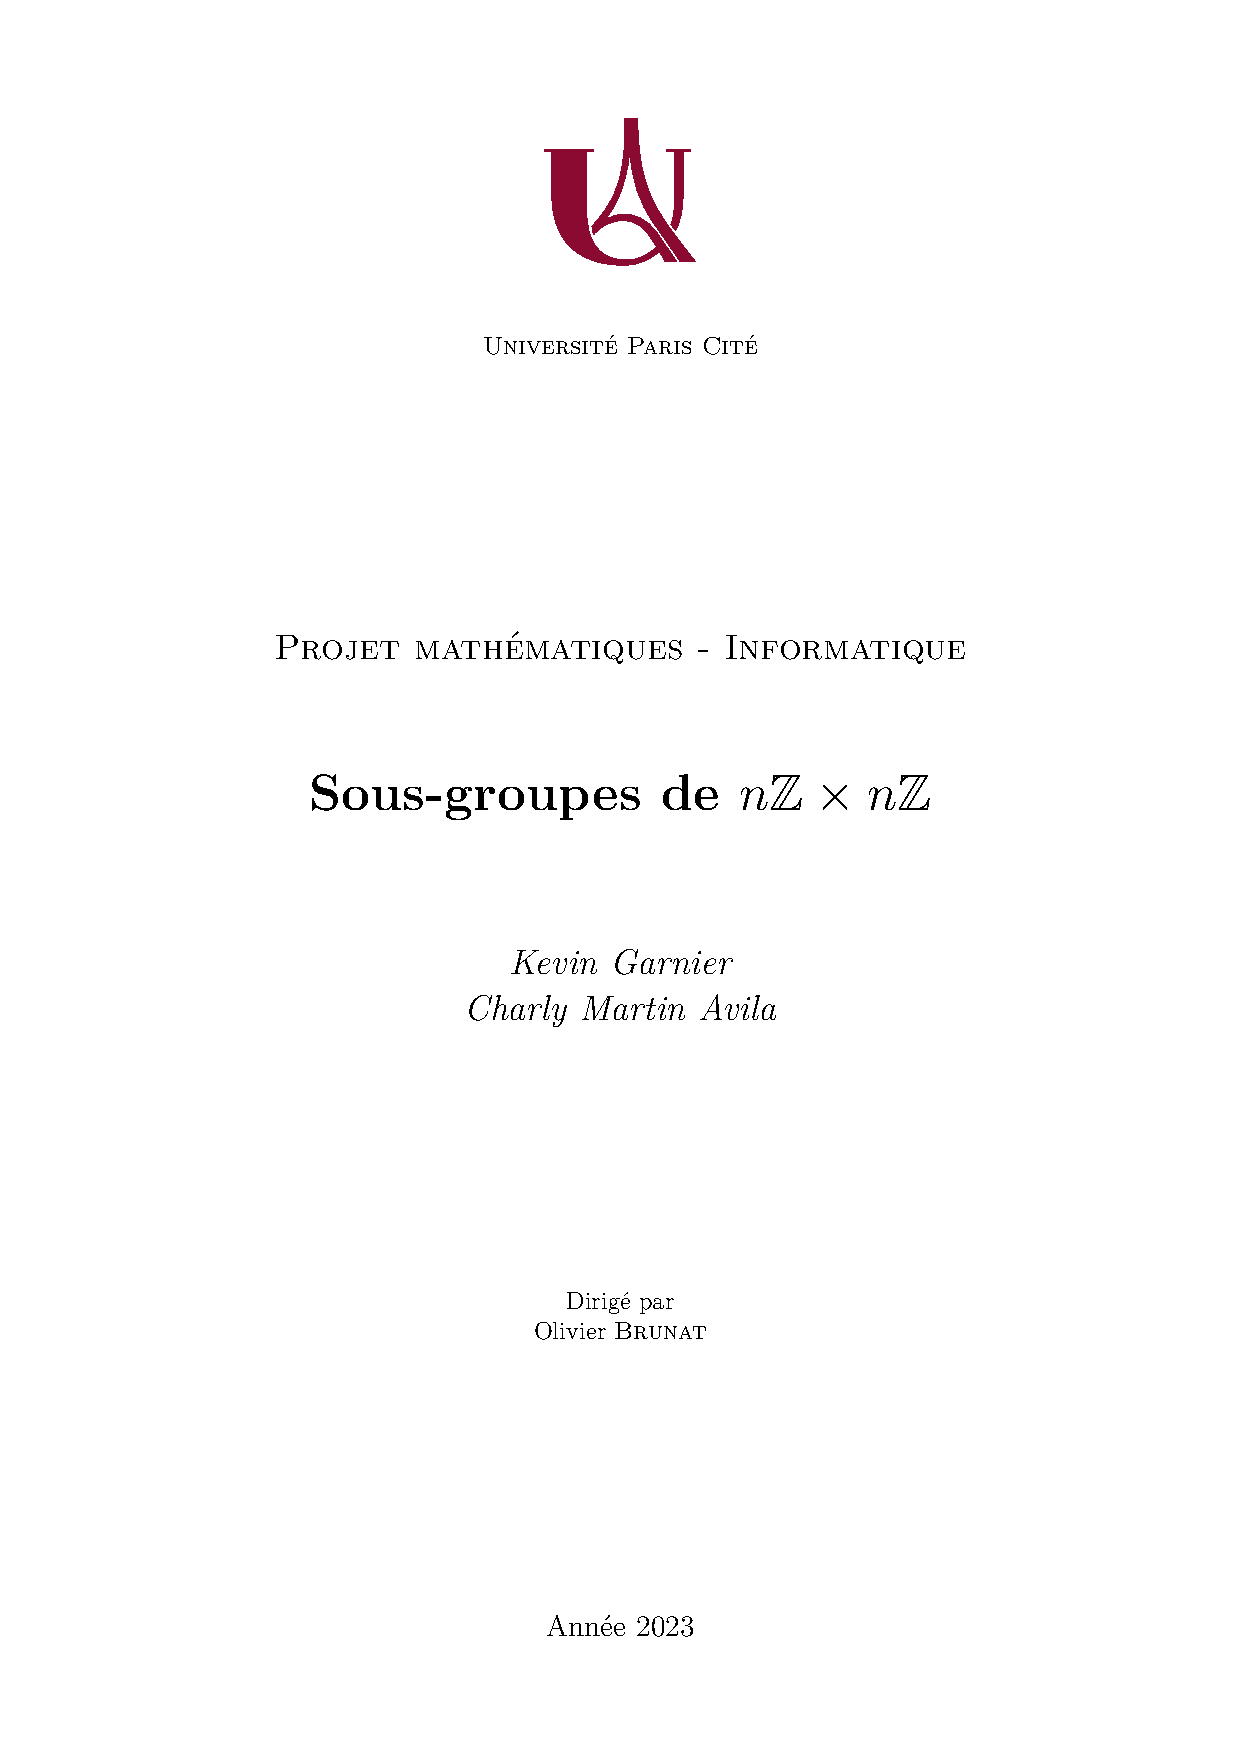
\includepdf{title.pdf}
\tableofcontents
\newpage

\section{Introduction}
	Il est très facile de décrire tous les sous-groupes d'un groupe cyclique
	d'ordre $n$ : il y en a exactement un par diviseur positif de $n$.
	Pourtant, étonnamment, décrire tous les sous-groupes d'un groupe abélien
	est en général un problème difficile.\\
	Dans ce projet, nous nous se proposons de considérer cette question pour le groupe $\ZZ$.

	D'un point de vue théorique, nous mettrons en avant la générations et la caractérisations de \\
	sous-groupes grâce aux vecteurs colonne des matrices à coefficients entier et en particulier aux formes
	normales de Hermite. Nous montrerons aussi une formule permettant de les compter.

	D'un point de vue pratique, nous créerons un programme \textsc{OCaml} capable de générer les\\
	sous-groupes de $\ZZ$ ainsi que leur treillis à partir d'un entier donné en paramètres.


\section{Quelques simplifications du problème}
% lemme des restes chinois, algorithme nombre premier, decomposition nombre premier
\subsection{Décomposition de $n$ en éléments irréductibles}
Nous pouvons tout d'abord simplifier le problème aux cas où $n = p^m$ avec $p$ un nombre premier
et $m \in \N$. En effet, soit
$$n = \prod_i^k p_i^{\alpha_i}$$
Par le théorème des restes chinois, on a
$$ \ZnZ \isom (\Z/p_i^{\alpha_i}\Z) \x \cdots \x (\Z/p_i^{\alpha_i}\Z)$$
En particulier,
\begin{equation*}
	\begin{split}
		\ZZ & \isom
		(\Z/p_i^{\alpha_i}\Z) \x \cdots \x (\Z/p_i^{\alpha_i}\Z) \x (\Z/p_i^{\alpha_i}\Z) \x \cdots \x (\Z/p_i^{\alpha_i}\Z)\\
			& \isom (\Z/p_i^{\alpha_i}\Z)^2 \x \cdots \x (\Z/p_i^{\alpha_i}\Z)^2
	\end{split}
\end{equation*}

En pratique, pour décomposer en entier en facteurs irréductibles, nous avons utilisé la procédure de
\textsc{$\rho$-Pollard} pour obtenir un diviseur de $n$:
\begin{verbatim}
fonction rho_pollard P x y k i d
  si d <> 1 Retourne d
  sinon
    x = P(x) mod n
    d = pgcd(|y - x|, n)
    Si i = k
      Alors Retourne rho_pollard loop P x x 2k (i + 1) d
    Sinon Retourne rho_pollard P x y k (i + 1) d
\end{verbatim}
Dans notre implémentation, $P(X) = X^2 - 1$.\\
Puis nous répétons la procédure jusqu'à que les diviseurs soient premier.
En triant et en regroupant les nombres premier, nous obtenons donc les différents $p^{\alpha_i}_i$

\subsection{Simplification des sous-groupes}
Soit \app{\varphi}{\Z^2}{\ZZ}{(a,b)}{(\bar a, \bar b)}
$\varphi$ est surjective par définition de la casse d'équivalence de a et b

\section{Matrices à coefficients entier et forme normales de Hermite}

% TODO : ajouter demo en rapport avec les matrice im AQ= im A etc
%

\section {Generation et Enumeration des sous-groupes}
%preuve sur la bonne forme de forme normale de Hermite
%preuve sur le calcul du nombre de sous-groupe

\section {Quelques résultats}

\end{document}
